\documentclass[preprint,12pt]{elsarticle}
\linespread{1}
\usepackage{amssymb}
\usepackage{lineno}
\usepackage[margin=0.5 in]{geometry}
\usepackage[utf8]{inputenc}
\usepackage{amsmath}
\usepackage{graphicx}
\usepackage{epstopdf}
\usepackage{lmodern}
\usepackage{caption}
\graphicspath{ {figures/} }

\newcommand{\exedout}{%
  \rule{0.8\textwidth}{0.5\textwidth}%
}
\begin{document}

\begin{frontmatter}

\title{FlexPass: Incentive Prompts for Reducing on-campus Parking Demand}

\author{Dounan Tang, Ziheng Lin,}

\address{University of California, Berkeley}

\begin{abstract}
%% Text of abstract

\end{abstract}


\begin{keyword}
Parking \sep Incentives \sep Randomized Controlled Trial \sep Casual Inference \sep 
%% keywords here, in the form: keyword \sep keyword

%% MSC codes here, in the form: \MSC code \sep code
%% or \MSC[2008] code \sep code (2000 is the default)
\end{keyword}

\end{frontmatter}

\section{Introduction} (7-25)
In order to reduce on-campus parking demand and create a more sustainable environment, a new parking pricing strategy is being proposed by the Parking and Transportation office of University of California, Berkeley. This parking pricing strategy, named FlexPass, is to be priced to provide an incentive to park less on working days, and preferably less than four working days per week during the hours 7 am to 6 pm. Before formally launching the FlexPass into the market, an experiment was conducted during 2015-Spring semester, Feb-1-2015 to Apr-30-2015, to test the treatment effect of this new strategy. Participants in the FlexPass study will be able to claim the rebate using a smartphone app. The rebates will accumulate over the semester and be added to their July 2015 paycheck. 

\section{Description of the FlexPass Study} 
The current parking pricing system at the University of California, Berkeley (UC Berkeley) is dominated by annual or monthly parking permits. Employees purchase an annual or monthly parking permit for a lump sum cost, then they will have the incentive to drive to campus every day, since the cost of parking is not affected by their days of parking on campus. The FlexPass study is being proposed to potentially reduce the demand of parking, which could also reduce the congestion and greenhouse gas emissions from cruising for parking, as well as to encourage mode choices other than driving alone. The study runs for 2015 Spring semester, 3 months beginning on February 1, 2015 and ending on April 30, 2015.

\subsection{Experimental Design}
Currently, there are more than 20 types of campus parking permits in UC Berkeley, this project will only target the current annual Central \textbf{C} Campus Permit and Faculty/Staff \textbf{F} Permit holders who constitute the vast majority of the regular users of campus parking. These parking permits allow holders to seek a parking space in parking garages or surface lots by the permit type. 'C' permits are available only to faculty and senior staff, \textbf{F} permits to other staff. To park on campus, permit holders are required to hang their permits on the rear-view mirror. Parking enforcement is conducted by UC Berkeley Parking and Transportation officers by checking these hang tags. The current price for \textbf{F} permit is \$95 per month while \$ 131 per month for \textbf{C} permit. Participants are only allowed to take part in this study if they have already purchased a \textbf{C} or \textbf{F} permit for the entire 2015 Spring semester. Enrolled participants will be assigned into two groups, rebate and control group, through a randomized controlled trial. If assigned to the control group, participants will only be required to install the FlexPass App and report parking behavior for the entire study period. They will keep their current permit. If assigned to the treatment group, they will be asked to turn in their current hang-tag and receive an alternate one, FlexPass permit, for the study period.  \\

Participants are able to report their daily parking choices on the FlexPass App, which is available for both Iphone and Android users. App interface is shown in figure \ref{fig:app_screens}. The default setting for every day will be “Parked on Campus”. Participants can change to not park on campus for today or tomorrow on the main interface, or for several days in the future through the calendar. If participants indicate that they will not park, they will also be asked to report what alternate mode would be taking or whether they would not be coming to campus. Participants can change their parking choices for a certain day in the study period, multiple times but only till 12 noon on that day. Participants' responses regarding whether or not parking on a certain day are uploaded to the server through the FlexPass App and then sent to parking enforcement officers. If assigned to treatment group, participants may be cited if park on campus after declaring that he will not. 

\begin{figure}[!htb]
\centering
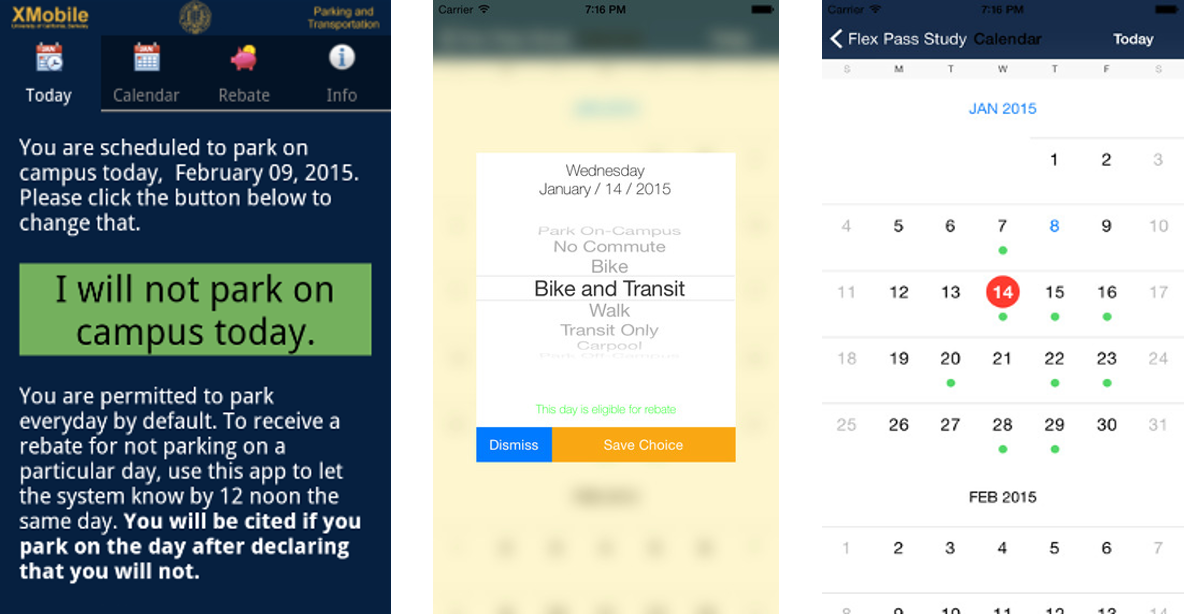
\includegraphics[scale=0.8]{app_screens.png}
\caption{FlexPass smartphone App interface. From left to right, (a) Main Screen, (b)Mode Reporting, (c) Calendar}
\label{fig:app_screens}
\end{figure}

There will be a guaranteed \$50 Amazon gift card just for participating and running the FlexPass App for the entire study period. Both group will report their daily commute modes while only rebate group is eligible for rebates which are based on their permit type and the number of working days (Mon to. Fri.) they park on campus in a given month. Rebate amounts are calculated as equation 1 below.

\[T = \max \{ \Theta  - D\delta ,0\} \]

where $D$ is the number of working days a certain participant parks on campus in a certain month and $T$ is the total rebates for that month. For that participant, the maximal rebate he or she can earn in that month is $\$\Theta$ ($\Theta$=95 for F permit holder while 131 for C permit). Every day that participant parks on campus, he or she will be changed a $\$\delta$ per day credit ($\delta$ =6 for F permit holder while 8 for C permit) until all credit has been used up. For example, as an F permit holder, if you park 12 workdays (approximately 3 work days a week), you will receive a rebate of \$23, if you park 13 days, you will receive a rebate of \$17 (i.e. \$23-\$6).\footnote{Detail description of the rebate calculation and a table of all possible rebate values can be found in the homepage of our study website https://gogreen.berkeley.edu/flexpass/.} Since participants will have already prepaid for their permit parking, the entire credit for three months will be refunded to them as a lump sum at the end of the study. 


\subsection{Sample Characteristics}

Our interested population consists of 4272 C\&F permit holders, and the enrollment was conducted through recruitment emails and postcards. 392 participants finished the sign-up procedure, where they responded to a few demographic, mobile technology and commute related questions. Then they were assigned into two groups through a randomized controlled trial, both group has sample size of 196. 

\section{Causal Analysis of the FlexPass Study}
To infer the treatment effect of the FlexPass, we proposed a box model as shown in figure \ref{fig:box_model}(a). For a certain participants indexed by $i$, his or her social economic characteristics, denoting as $X_i$ on his or her ticket, are observed through the entry survey. The ticket in the box also contains the treatment respond vector $Y_i^T$ and control respond vector $Y_i^C$. $Y_i^T$ and $Y_i^C$ is both constructed by 64 binary variables, denoting as $Y_{ij}^t$ and $Y_{ij}^c$, representing daily parking choices,which equals 1 if participant $i$ did not park on campus on day $j$ and 0 otherwise. 392 samples were drawn from the box of 4272 C\&F permit holders and assigned into treatment group and control group randomly. Let $T_i$ represents group assignment which equals 1 if assigned into treatment group and 0 otherwise. If $T_i=1$, $Y_i^T$ would be potentially observable while we observe $Y_i^C$ when $T_i=0$. Denote the overall parking choices as $\mathbf{Y}$, which is a $392\times 64$ 0-1 matrix. Under the week null hypothesis $H_0$, there is no treatment effect in the population level, which assumes the FlexPass has no effect on reducing on-campus parking demand. The purpose of our causal analysis is the evaluate the size and variance of the treatment effect $\overline {\sum\limits_j \mathbf{{{Y^t}_{ij}}} }  - \overline {\sum\limits_j \mathbf{{{Y^c}_{ij}}} } $ to decide whether we can reject the null hypothesis at certain confidence level. However, problem arisen during the study as not all $Y_{ij}$s are observed, which causes biases in causal analysis. \\

In this section, missing data and dropout problems will be addressed. The missing data will be imputed by a mixed latent factor model while dropout bias will be compensated through selection model. The result of casual analysis will then be discussed.    

\begin{figure}[!htb]
\centering
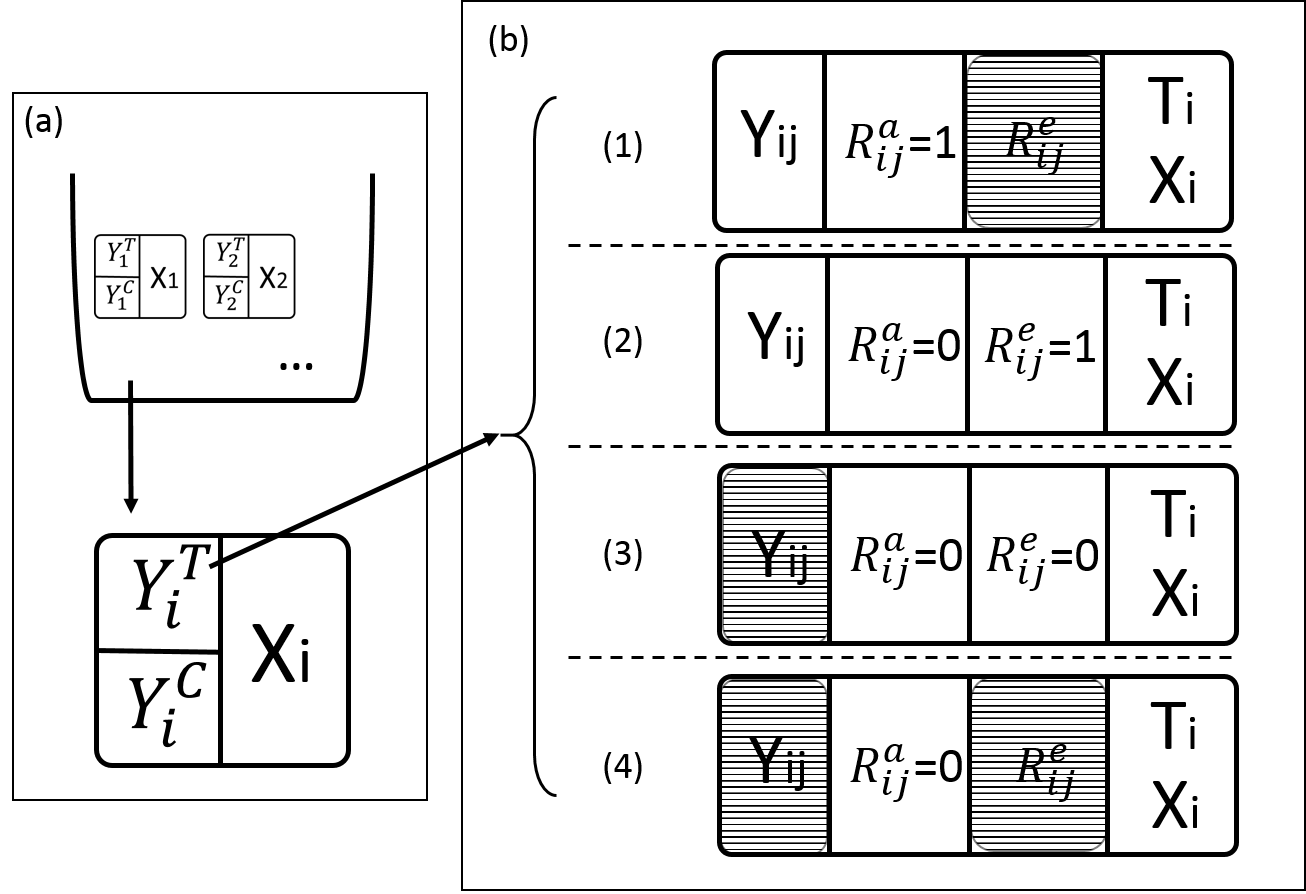
\includegraphics[scale=0.4]{box_model.png}
\caption{Box model for causal analysis}
\label{fig:box_model}
\end{figure}

\subsection{Dropouts, Missing reports and Data Descriptions}

In order to do the enforcement, participants assigned to the rebate group were required to pick up their new FlexPass hang-tap at Parking and Transportation office. Only 149 participants exchanged their hang-tap and the rest 47 within the rebate group dropped out during this process. There were two participants dropped out after picked up the FlexPass because of switching to carpool and being pregnant, which further reduced the size of rebate group to 147. The situation for control group is more complicated. As there is no incentives for them to report daily commute modes, from the beginning (Feb-01-2015) to the end (Apr-31-2015) there are 80 participants in the control group have not reported any mode choices through our smartphone App. Even with participants who have reported some choices, they may still under report the number of not-park-on-campus days, which leads to an overestimation of the treatment effect. Therefore, instead of respond $Y_{ij}$, we additionally define, for each occasion j, an indicate $R_{ij}^a$, which equals 1 if participant $i$ reported day $j$'s parking behavior through smartphone App and 0 if participant $i$ didn't use the App on day $j$. We then partition $Y_i$ into two sub-vectors such that $Y^o_i$ is the vector containing those $Y_{ij}$ for which $R_{ij}^a=1$ and $Y^m_i$ contains the remaining components. $Y^m_i$ is referred to missing reports. As the default setting on the App is "Park on Campus". We are expected to see that $Y^m_i$ and $Y^o_i$ is distinct. To further understand the missing report process, we have sent out some weekly follow-up emails to the participants who have not reported any commute mode choices in the previous week to ask how they came to campus each weekday. Emails are only send out in the .... weeks. For each occasion j, another indicator is defined as $R_{ij}^e$, which equals 1 if participant $i$ reported day $j$'s parking behavior through email and 0 otherwise.
\\
 
Respond vector $Y_i$ are measured through both App and email system, all possible outcomes for $Y_{ij}$ are then illustrated in figure \ref{fig:box_model}(b), where the shaded region means not observable. In situation (1), participant i report day j's parking choice through the App, where $Y_{ij}$ is observed and on email will be sent. In situation(2) , participant i didn't use the App on day j and an email will be sent to i. He or she answered the email and thus $Y_{ij}$ is observed. In situation(3), $Y_{ij}$ is not observed as participant i didn't answer the email. As emails are only sent out for six weeks, situation(4) may also happen, where participants i would not receive any email even he didn't use the App for certain days. Or participants i belongs to treatment group but dropped out when asked to change hang tag. He or she will uninstall the App and never appears in the email list. Noticeably, all $Y^o_i$ is observed in this study by definition and part of $Y^m_i$ is measured in situation (2). If $Y_i$ only contains $Y_{ij}$ generated in situation (3) and (4), participants i is regarded as 'Dropout Participants'. Otherwise, complete data $Y_i$ will be recovered from $Y_{ij}$ observed in situation (1) and (2).

longitudinal data

email data

\subsection{Recover Missing Reports} 
Missing not at random(MNAR)\\

In the most simple case, $Y_{ij}$ is fitted by a linear model as
\[{Y_{ij}} = {\mathbf{U_i}}'{\mathbf{V_j}} + {\varepsilon _{ij}}\]
where $\mathbf{U_i}$ and $\mathbf{V_j}$ are L dimension vectors. In models based on concrete attributes, $\mathbf{U_i}$ may be L distinct characteristics for participants $i$, e.x. age, income and gender, while $\mathbf{V_j}$ may be corresponding coefficient vectors of day $j$, e.x. $\mathbf{V_j}$ may be different for Fridays and Mondays. However, if instead of interpretive ability we care about predicting accuracy, there will be better candidates of $\mathbf{V_j}$ than social economic features, which give rise to Latent Factor Model(LFM).\\     

When $\varepsilon _{ij}$ is independent and identically Gaussian distributed, the estimated parking respond matrix $\hat{Y}$ can be expressed by $\mathbf{U}'\mathbf{V}$, where $\mathbf{U}$ and $\mathbf{V}$ is a $M\times L$ and $N\times L$ matrices respectively. Let ${\left\| . \right\|_F}$ denotes Frobenius norm, to maximize the likelihood function equals to solve:

\[{\min _{rank(\widehat {\mathbf{Y}}) \leqslant {\text{L}}}}{\left\| {{\mathbf{Y - }}\widehat {\mathbf{Y}}} \right\|_F}\]

whose solution is essentially a singular value decomposition of $\mathbf{Y}$. 

\[{Y_{ij}} = (1 - {R^a}_{ij}){\alpha ^m}_i + {R^a}_{ij}{\alpha ^o}_i + {\beta _j} + {{\mathbf{U}}_{\mathbf{i}}}{\mathbf{'}}{{\mathbf{V}}_{\mathbf{j}}} + {\varepsilon _{ij}}\]


\begin{figure}[!htb]
\centering
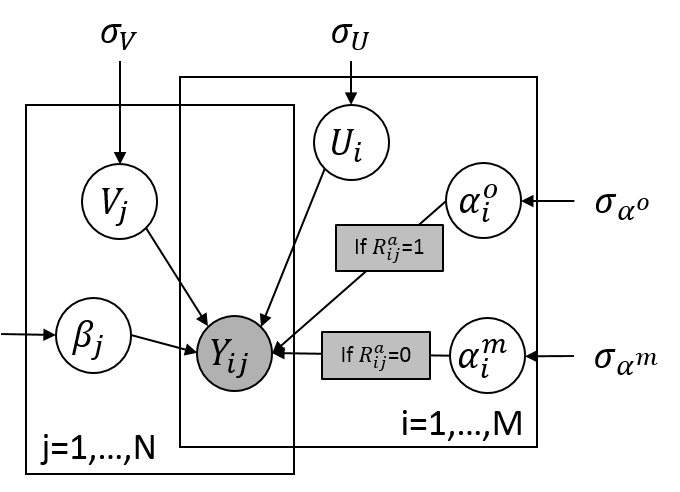
\includegraphics[scale=0.6]{MLFM.png}
\caption{Graphic Model for Mixed Latent Factor Model}
\label{fig:MLFM}
\end{figure}

\subsection{Compensate Dropout Bias} (7-24)

\section{Conclusion} (7-24)

\end{document}
